\documentclass{article}
\usepackage[utf8]{inputenc}
\usepackage{graphicx}
\usepackage[spanish,es-tabla]{babel}
\usepackage{amsmath}
\usepackage[a4paper,margin=1in,footskip=.5cm]{geometry}
\usepackage{subcaption}
\setlength\headheight{30pt} 
\usepackage{fancyhdr}
\usepackage{amssymb}
\usepackage[hidelinks]{hyperref}
\usepackage{mathtools}
\usepackage[table,xcdraw]{xcolor}
\usepackage[backend=bibtex]{biblatex}
\usepackage{csquotes}
\usepackage{float}
\usepackage{listings}
\usepackage{xcolor}
\usepackage{circuitikz}


\definecolor{codegreen}{rgb}{0,0.6,0}
\definecolor{codegray}{rgb}{0.5,0.5,0.5}
\definecolor{codepurple}{rgb}{0.58,0,0.82}
\definecolor{backcolour}{rgb}{0.95,0.95,0.92}

\lstdefinestyle{mystyle}{
    backgroundcolor=\color{white},   
    commentstyle=\color{codegreen},
    keywordstyle=\color{magenta},
    numberstyle=\tiny\color{codegray},
    stringstyle=\color{codepurple},
    basicstyle=\ttfamily\small,
    breakatwhitespace=false,         
    breaklines=true,                 
    captionpos=b,                    
    keepspaces=true,
    numbersep=5pt,                  
    showspaces=false,                
    showstringspaces=false,
    showtabs=false,                  
    tabsize=2
}

\lstset{style=mystyle}



\hypersetup{
colorlinks = true,
urlcolor=blue,
linkcolor = black
}
\title{TP1_EAIII}
\author{FACUNDO NAHUEL GALVAGNO}
\date{April 2025}

\begin{document}

\renewcommand{\figureautorefname}{Fig.}
\renewcommand{\tableautorefname}{Tab.}
\renewcommand{\equationautorefname}{Ec.}

\pagestyle{fancy}
\fancyhf{}
\fancyhead[R]{\includegraphics[width=8cm]{fig/color_UNC-FCEFyN.png}}
\fancyhead[L]{Electrónica Analógica III - Acopladores}
\fancyfoot[R]{\thepage}
\renewcommand{\headrulewidth}{0.1pt}
% agregamos la caratula
\begin{titlepage}

\begin{center}
    \includegraphics[width=15cm]{fig/color_UNC-FCEFyN.png} 
    \\[1cm]
    \vspace{5pt}
    \ \LARGE Universidad Nacional de Córdoba\\[0.5cm] 
    \large Facultad de Ciencias Exactas, Físicas y Naturales \\[0.5cm] 
    \large Electrónica Analógica III
    \\[0.2cm]
    \large TP N° 1
    \\[0.2cm]
    \large Acopladores
    \\[0.2cm]
    \vspace{360pt}
    \begin{table}[!h]
    \centering
    \begin{tabular}{ll}
    \multicolumn{1}{c}{Nombre} & \multicolumn{1}{c}{DNI} \\
    Galvagno Facundo Nahuel& 40815088 \\
    
    \end{tabular}
    \end{table}
\vfill Córdoba, República Argentina\\ \today
\end{center}

\end{titlepage}
\newpage

\tableofcontents
\newpage

\section{Introducción}

Este informe presenta el proceso de diseño, construcción y medición de un circuito doblemente sintonizado con adaptación de impedancias en una configuración RLC en paralelo. El objetivo es lograr una frecuencia de resonancia de 18 MHz y asegurar una correcta adaptación de las impedancias tanto en la entrada como en la salida.

Se llevaron a cabo los cálculos necesarios para determinar los valores óptimos de los componentes del circuito, incluyendo los capacitores y un inductor de núcleo de aire, con el propósito de cumplir con los requisitos de frecuencia de resonancia y adaptación de impedancias. Además, se diseñó y fabricó el inductor de núcleo de aire considerando la inductancia necesaria, así como las restricciones de espacio y los materiales disponibles.

Se utilizó Python como ayuda de cálculo numérico y LTSpice para las correspondientes simulaciones.


\newpage

\section{Diseño}
Si se parte del circuito típico para un resonador LC paralelo, el mismo resonará a una frecuencia $f_0$ dada por

$$
f_0 = \frac{1}{2\pi\sqrt{LC}}
$$

\begin{figure}[H]
    \centering
    \includegraphics[width=0.5\linewidth]{fig/lcparalelo.png}
    \caption{circuito LC paralelo}
    \label{fig:enter-label}
\end{figure}

Además

$$
Q = \frac{f_0}{BW} = \frac{R_T}{X_L}   
$$

Donde $BW$ representa el ancho de banda del circuito. La resistencia total $R_T$ del circuito esta definida por la impedancia de entrada $R_a$, la impedancia de salida $R_L$ y la resistencia de pérdida del inductor $R_P$. Para este análisis se desprecia la pérdida en los capacitores. En este circuito, no podemos elegir el ancho de banda, puesto que el mismo depende de las impedancias de entrada y salida.

$$
R_T = R_a//R_p//R_L
$$

Para poder elegir de manera independiente el ancho de banda y lograr adaptar impedancias de entrada y salida, se debe de adoptar ciertas modificaciones en el circuito. Si se divide el capacitor $C$ en cuatro capacitores, se tiene el siguiente circuito.

\begin{figure}[H]
    \centering
    \includegraphics[width=0.5\linewidth]{fig/circuito.png}
    \caption{acoplador}
    \label{fig:enter-label}
\end{figure}

Para no alterar el la frecuencia de resonancia $f_0$ del circuito, se debe procurar que la capacidad equivalente se mantenga igual, es decir

$$
C = \frac{1}{1/C_1+1/C_2} + \frac{1}{1/C_3+1/C_4}
$$

De esta forma, la impedancia de entrada y de salida son adaptadas por un factor de transformación, dados por los pares de capacitores $C_1,C_2$ y $C_3,C_4$, para $R_a$ y $R_L$ respectivamente. 

\subsection{Transformador Capacitivo}

Si se realiza el analisis de la impedancia en una de las ramas, se tiene que la admitancia equivalente $Y_e$ esta dada por

\begin{figure}
    \centering
    \includegraphics[width=0.5\linewidth]{fig/divcap.png}
    \caption{circuito equivalente del divisor capacitivo}
    \label{fig:enter-label}
\end{figure}

$$
Y_{s1} = \frac{1}{R_e}+\frac{1}{XC_2} 
$$
$$
Y_e = \frac{Y_{s1}*1/XC_1}{Y_{s1}+1/XC_1}
$$
$$
Y_e = \frac{1+jwC_2R}{1+jw(C_1+C_2)R}jwC_1
$$

Multiplicando por el conjugado y reordenando, obtenemos
$$
Y_e = \frac{1-jw(C_1+C_2)R+jwC_2R+w^2C_2+R^2(C_1+C_2)}{1+w^2(C_1+C_2)R^2}jwC_1
$$

$$
Y_e = \frac{w^2C_1^2R+jwC_1[1+w^2C_2R^2(C_1+C_2)]}{1+w^2R^2(C_1+C_2)^2}
$$

Pero si tenemos que $1<<w^2R^2(C_1+C_2)^2$ y $1<<1+w^2C_2R^2(C_1+C_2)]$ por ser $w$ muy grande

$$
Y_e = \frac{w^2C_1^2R+jw^3C_1C_2R^2(C_1+C_2)}{w^2R^2(C_1+C_2)^2}
$$

Si separamos los terminos reales de los terminos complejos, obtenemos

$$
Y_e = \frac{C_1^2}{(C_1+C_2)^2}*\frac{1}{R}+jw*\frac{C_1C_2}{C_1+C_2}
$$

Entonces

$$R_e = R\frac{C1+C2}{C1}^2=R*(1+\frac{C_2}{C_1})^2$$

$$
C_e = \frac{C_1*C_2}{C_1+C_2}
$$

Por lo tanto, podemos reescribir las impedancias equivalentes $R'_a$ y $R_L'$ como

$$
R_a' = \left( 1 + \frac{C_2}{C_1} \right)^2 R_a \\
$$
$$
R_L' = \left( 1 + \frac{C_3}{C_4} \right)^2 R_L
$$

A partir de las impedancias equivalentes sobre $L$, ahora $R_T$ está dada por

$$
R_T = R_a'//R_p'//R_L
$$

\subsection{Selección de $L$}

Puesto que existen infinitos pares de $L$ y $C$ que satisfagan la condición de $f_0$, se deben plantear ciertos criterios a la hora de elegir los valores correspondientes. Para una determinada $f_0$, utilizar capacidades muy grandes resulta en inductores muy pequeños y viceversa. Se plantea conformar iterativamente una gran cantidad de pares LC para satisfacer las especificaciones de diseño. El cálculo de $L$ se realizó asumiendo ciertos parámetros físicos, como la sección del cobre y el paso de las espiras.

Partiendo de los requerimientos de diseño

\begin{enumerate}
    \item $f_0 = 18 MHz$
    \item $BW = 1MHz$
    \item $Z_{in}=50\Omega$
    \item $Z_{Out} = 1K\Omega$
\end{enumerate}

Se calcularon de forma tabulada varios pares LC. Los mismos se encuentran detallados en el archivo de \textit{jupyter notebook} llamado \textit{tabla.ipynb}.

En el código, se definen los siguientes parámetros iniciales:
\begin{itemize}
    \item \( f_o = 18 \) MHz: Frecuencia de operación.
    \item \( d = 0.15 \) cm: Diámetro del conductor.
    \item \( D = 1.65 \) cm: Diámetro del núcleo.
    \item \( s = d \): Separación entre espiras (igual al diámetro del conductor).
    \item \( p = s + d \): Paso de la espira.
    \item \( N_s = \frac{1}{s + d} \): Número de vueltas por cm.
    \item \( Q_c = 10 \): Factor de calidad de acoplamiento.
    \item \( R_g = 50 \) \( \Omega \): Resistencia del generador.
    \item \( R_l = 1000 \) \( \Omega \): Resistencia de carga.
\end{itemize}

Se ejecuta un bucle que varía la capacitancia en pasos de 10 pF, y para cada valor se obtiene $K$ y $l/D$ a partir de una interpolación de la curva del factor de Nagaoka tabulado. El número de vueltas del inductor de núcleo de aire es calculado a partir de $Ns$ y $l$.

\begin{figure}[H]
    \centering
    \includegraphics[width=0.5\linewidth]{fig/interpolacion.png}
    \caption{interpolación de los valores tabulados del factor de Nagaoka}
    \label{fig:enter-label}
\end{figure}

\subsection{Selección de Capacitores}

Una vez obtenidos los parámetros del inductor, tambien se calcula la combinación necesaria de capacitores $C_1$, $C_2$, $C_3$ y $C_4$ a partir de la resistencia de pérdida del inductor, la impedancia de entrada y salida y el ancho de banda.
$$
    C_2 = \frac{C}{2} \sqrt{\frac{R_{ap}}{R_g}}
$$
$$
    C_1 = \frac{C}{2} \times \frac{C_2}{C_2 - C/2} 
$$
$$
    C_4 = \frac{C}{2} \sqrt{\frac{R_{Lp}}{R_l}} 
$$
$$
C_3 = \frac{C}{2} \times \frac{C_4}{C_4 - C/2} 
$$

Los capacitores utilizados deben tener valores realizables, esto quiere decir que el inductor se descarta si sus parámetros generan valores de capacitores negativos o demasiado pequeños.

\subsection{Parámetros Finales}
Los valores finales para los componentes a utilizar son:
\[
\begin{array}{|c|c|c|}
\hline
\textbf{Parameter} & \textbf{Value} & \textbf{Unit} \\
\hline
C & 150.000 & \text{pF} \\
L & 521.200 & \text{nH} \\
N_s & 3.333 & \text{vueltas/cm} \\
K & 10.442 & \text{-} \\
l_d & 1.4478908999912352 & \text{} \\
l & 2.389 & \text{cm} \\
N & 7.963 & \text{vueltas} \\
Q & 449.753 & \text{-} \\
X_L & 58.946 & \Omega \\
R_p & 26.511 & K\Omega \\
R_t & 589.463 & \Omega \\
R_{ap} & 1.179 & K\Omega \\
R_{Lp} & 1.234 & K\Omega \\
C_1 & 94.451 & \text{pF} \\
C_2 & 364.183 & \text{pF} \\
C_3 & 752.132 & \text{pF} \\
C_4 & 83.307 & \text{pF} \\
C_t & 150.000 & \text{pF} \\
\hline
\end{array}
\]
\newpage

\section{Simulación}
A partir de los componentes seleccionados, se simula el circuito con \textit{LTSpice}.

Para que la simulación se asemeje lo más posible al circuito realizable, se seleccionarán capacitores de valores normalizados lo más cercano posible a los calculados, es decir

\[
\begin{array}{|c|c|c|}
\hline
\textbf{Parameter} & \textbf{Value (F)} & \textbf{Valor comercial} \\
\hline
C_1 & 94.451E-12 & 100 \, \text{pF} \\
C_2 & 364.183E-12 & 330 \, \text{pF} \\
C_3 & 752.132E-12 & 680 \, \text{pF} \\
C_4 & 83.307E-12 & 82 \, \text{pF} \\
\hline
\end{array}
\]

\subsection{Respuesta en Frecuencia}

Se mide la salida sin $R_L$ para disminuir el ancho de banda, obteniendo $f_0 = 17.82 MHz$ a partir del cursor.

\begin{figure}[H]
    \centering
    \includegraphics[width=0.5\linewidth]{fig/bode.png}
    \caption{respuesta en frecuencia del acoplador simulado}
    \label{fig:enter-label}
\end{figure}

\subsection{Impedancia de Entrada y Salida}

La impedancia de entrada está dada por la diferencia entre la caida de tensión en la entrada del circuito con y sin el acoplador conectado.

\begin{figure}[H]
    \centering
    \includegraphics[width=0.5\linewidth]{fig/zin.png}
    \caption{medición de la impedancia de entrada}
    \label{fig:enter-label}
\end{figure}

Se observa que la tensión en la entrada cae a aproximadamente la mitad al conectar el acoplador para la frecuencia de resonancia, lo cual indica una impedancia correctamente adaptada. Matemáticamente, esto es

$$
Z_{in} = \frac{R_a}{Vg/Vi-1} = \frac{50\Omega}{3V/1.56-1} = 54.16\Omega
$$

La impedancia de salida se puede medir al contrastar la caída de tensión sobre la salida del acoplador al conectar y desconectar la carga.

\begin{figure}[H]
    \centering
    \includegraphics[width=0.5\linewidth]{fig/zo2.png}
    \caption{medición de la tensión de salida con carga}
    \label{fig:enter-label}
\end{figure}

\begin{figure}[H]
    \centering
    \includegraphics[width=0.5\linewidth]{fig/zout.png}
    \caption{medición de la tensión de salida sin carga}
    \label{fig:enter-label}
\end{figure}


$$
Z_{out} = R_L(\frac{V_O}{V_L}-1)= 1K\Omega(\frac{11.96V}{5.8V}-1)=1.02K\Omega
$$

\subsection{Ancho de Banda}
A partir de los 3db de atenuación en la carga del acoplador, se tiene

\begin{figure}[H]
    \centering
    \includegraphics[width=0.5\linewidth]{fig/bws.png}
    \caption{ancho de banda en simulador}
    \label{fig:enter-label}
\end{figure}

$$
BW = 18.76MHz - 16.90MHz = 1.65MHz
$$




\newpage

\section{Implementación}
Se realiza la implementación del acoplador sobre un PCB. La inductancia es fabricada según las especificaciones desarrolladas anteriormente.

\begin{figure}[H]
    \centering
    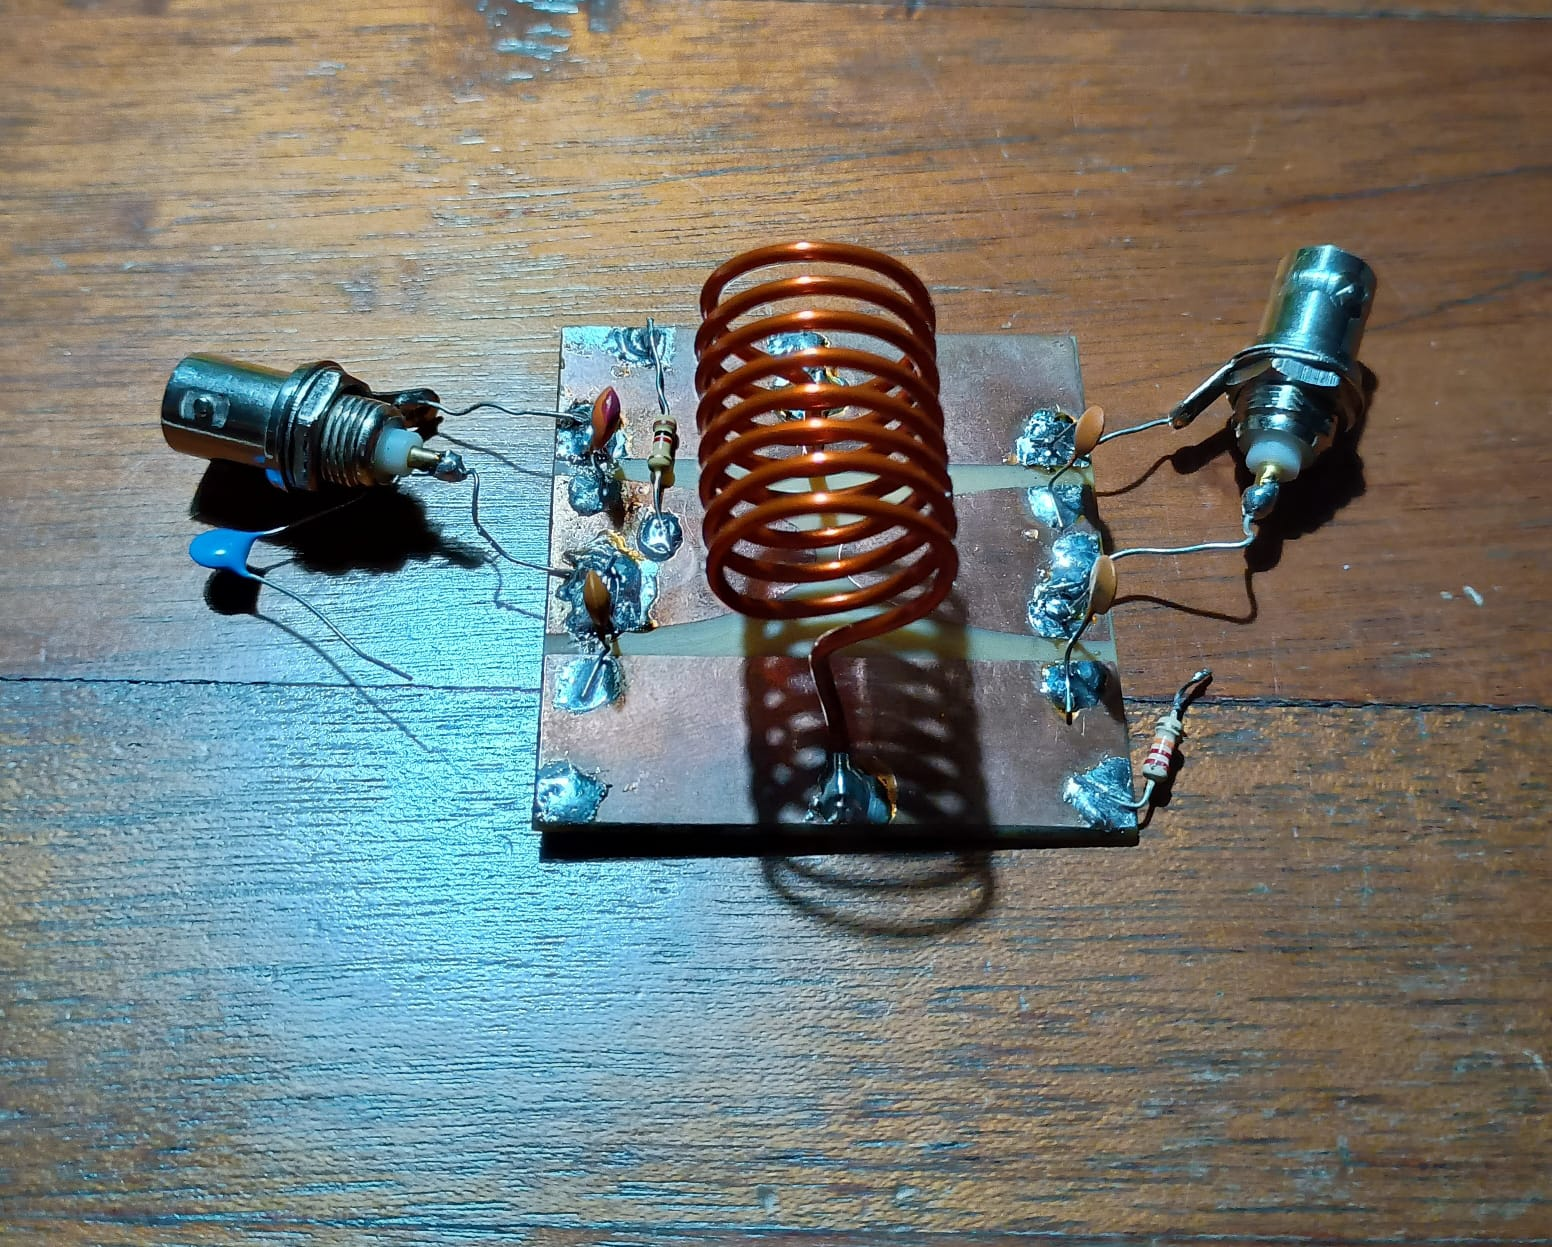
\includegraphics[width=0.5\linewidth]{fig/pcb.png}
    \caption{acoplador montado en PCB}
    \label{fig:enter-label}
\end{figure}

\subsection{Respuesta en Frecuencia}
Para medir $f_0$ sobre el circuito implementado, se debe de realizar una medición indirecta. Esto se debe a que el instrumental (generador de onda, osciloscopio, cables, etc) introduce una capacidad en paralelo con el circuito, modificando el valor de $C$. También se debe medir con una resistencia en serie que limite la corriente que entrega el generador, puesto que el circuito en resonancia tiene una resistencia muy baja, que puede ocasionar la destrucción del mismo.

\begin{figure}[H]
    \centering
    \includegraphics[width=0.5\linewidth]{fig/esqm.png}
    \caption{esquema de medición del circuito}
    \label{fig:enter-label}
\end{figure}

La resistencia $R_T$ se encuentra en el orden de la resistencia de pérdida $R_P$.

A partir de medir la caída de tensión en el acoplador, se encuentra que la frecuencia de resonancia $f'_0$ 

\begin{figure}[H]
    \centering
    \includegraphics[width=0.5\linewidth]{oscilo/SDS00003.jpg}
    \caption{caída de tensión en el acoplador en $f'_0$}
    \label{fig:enter-label}
\end{figure}
$$
f'_0 = 12.5MHz
$$

Como la capacidad $C_X$ agregada por el instrumental es indefinida, realizamos una segunda medición, agregando en paralelo con el osciloscopio una capacidad $C_F$ de $68pF$.

\begin{figure}[H]
    \centering
    \includegraphics[width=0.5\linewidth]{fig/ctest.png}
    \caption{se agrega una capacidad conocida $C_F$}
    \label{fig:enter-label}
\end{figure}

Se mide la frecuencia de resonancia $f''_o$.

\begin{figure}[H]
    \centering
    \includegraphics[width=0.5\linewidth]{oscilo/SDS00004.jpg}
    \caption{caída de tensión en el acoplador en $f''_0$}
    \label{fig:enter-label}
\end{figure}

$$
f'_0 = 11.0MHz
$$

Finalmente, se procede a calcular la capacidad inducida por el instrumental $C_X$.

$$
f'_0 = \frac{1}{2\pi\sqrt{L(C+C_X}}
$$

$$
f''_0 = \frac{1}{2\pi\sqrt{L(C+C_X+C}}
$$

Realizando el cociente entre $f'_{0}$ y $f''_{0}$ y elevando al cuadrado ambos términos se obtiene

$$
{\frac{f'_{0}}{f''_{0}}^2} = \frac{C+C_X+C_F}{C+C_X}
$$

Reordenando y reemplazando los valores obtenidos

$$
C_X = \frac{C({f''_{0}}^2-{f'_{0}}^2)+C_F*{f''_{0}}^2}{{f'_{0}}^2-{f''_{0}}^2} = 129.46pF
$$

De este valor, se puede despejar el valor del inductor

$$
L = {\frac{1}{2\pi*f'_0}}^2*1/(C+C_X) = 511nHy
$$

Por lo tanto, la frecuencia de corte del circuito medido es

$$
f_0 = \frac{1}{2\pi\sqrt{LC}} = 18.18 MHz
$$

\section{Impedancia de Entrada y Salida}

De forma análoga a la realizada en la simulación, la impedancia de entrada está dada por la diferencia entre la caída de tensión en la entrada del circuito con y sin el acoplador conectado.

\begin{figure}[H]
    \centering
    \includegraphics[width=0.5\linewidth]{oscilo/SDS00010.jpg}
    \caption{salida del generador}
    \label{fig:enter-label}
\end{figure}

\begin{figure}[H]
    \centering
    \includegraphics[width=0.5\linewidth]{oscilo/SDS00011.jpg}
    \caption{medición de la impedancia de entrada}
    \label{fig:enter-label}
\end{figure}

Se observa que la tensión en la entrada cae a aproximadamente la mitad al conectar el acoplador para la frecuencia de resonancia, lo cual indica una impedancia correctamente adaptada. Matemáticamente, esto es

$$
Z_{in} = \frac{R_a}{Vg/Vi-1} = \frac{50\Omega}{2.72V/1.16-1} = 40.66\Omega
$$

La impedancia de salida se puede medir al contrastar la caída de tensión sobre la salida del acoplador al conectar y desconectar la carga.

\begin{figure}[H]
    \centering
    \includegraphics[width=0.5\linewidth]{oscilo/SDS00018.jpg}
    \caption{medición de la tensión de salida con carga}
    \label{fig:enter-label}
\end{figure}

\begin{figure}[H]
    \centering
    \includegraphics[width=0.5\linewidth]{oscilo/SDS00017.jpg}
    \caption{medición de la tensión de salida sin carga}
    \label{fig:enter-label}
\end{figure}


$$
Z_{out} = R_L(\frac{V_O}{V_L}-1)= 1K\Omega(\frac{9.68V}{5.44V}-1)=0.77K\Omega
$$

\subsection{Ancho de Banda}
A partir de los 3db de atenuación en la carga del acoplador, se tiene

\begin{figure}[H]
    \centering
    \includegraphics[width=0.5\linewidth]{oscilo/SDS00021.jpg}
    \caption{límite inferior de ancho de banda}
    \label{fig:enter-label}
\end{figure}

\begin{figure}[H]
    \centering
    \includegraphics[width=0.5\linewidth]{oscilo/SDS00022.jpg}
    \caption{límite superior de ancho de banda}
    \label{fig:enter-label}
\end{figure}


$$
BW = 14.17MHz - 12.85MHz = 1.32MHz
$$


\subsection{Resistencia de Pérdida del Inductor, Qc y Qd}

A partir de la medición de $f'0$, en resonancia poseemos un divisor resistivo conformado por $R_a$, $R_T$ y $R_P$.

\begin{figure}
    \centering
    \includegraphics[width=0.5\linewidth]{fig/rp.png}
    \caption{esquema para la medición de $R_p$}
    \label{fig:enter-label}
\end{figure}

Entonces

$$
R_P = \frac{R_a+R_T}{V_i/V_o-1} = 22K\Omega
$$

A su vez, de los parámetros obtenidos podemos calcular

$$
Q_c = \frac{f_o}{BW} = 13.71
$$
$$
Q_d = \frac{R_P}{2\pi L} = 379,30 
$$



\newpage

\section{Comparación y Conclusiones}
A partir del diseño y la implementación del circuito, se logró realizar un acoplador cercano a las especificaciones requeridas.

La siguiente tabla refleja los resultados esperados, contra los obtenidos en simulación e implementación.

\begin{table}[h]
    \centering
    \begin{tabular}{|c|c|c|c|}
        \hline
        \textbf{Parámetro} & \textbf{Simulación} & \textbf{Medición} & \textbf{Diferencia (\%)} \\
        \hline
        Frecuencia de resonancia ($f_0$) [MHz] & 17.82 & 18.18 & 2.02\% \\
        \hline
        Impedancia de entrada ($Z_{in}$) [$\Omega$] & 54.16 & 40.66 & 24.88\% \\
        \hline
        Impedancia de salida ($Z_{out}$) [$\Omega$] & 1020 & 770 & 24.51\% \\
        \hline
        Ancho de banda (BW) [MHz] & 1.65 & 1.32 & 20\% \\
        \hline
    \end{tabular}
    \caption{Comparación entre valores simulados y medidos}
    \label{tab:sim_vs_med}
\end{table}

\begin{table}[h]
    \centering
    \begin{tabular}{|c|c|c|c|}
        \hline
        \textbf{Parámetro} & \textbf{Medición} & \textbf{Requisito de Diseño} & \textbf{Error con Medición (\%)} \\
        \hline
        Frecuencia de resonancia ($f_0$) [MHz] & 18.18 & 18.00 & 1.00\% \\
        \hline
        Impedancia de entrada ($Z_{in}$) [$\Omega$] & 40.66 & 50.00 & 18.68\% \\
        \hline
        Impedancia de salida ($Z_{out}$) [$\Omega$] & 770 & 1000 & 23\% \\
        \hline
        Ancho de banda (BW) [MHz] & 1.32 & 1.50 & 12.00\% \\
        \hline
    \end{tabular}
    \caption{Comparación entre valores medidos y requisitos de diseño}
    \label{tab:med_vs_req}
\end{table}

Existen discrepancias del orden del 20\% aproximadamente, sobretodo en las mediciones de las impedancias y el ancho de banda.

Puesto que estas variables estan estrictamente relacionadas con $R_T$. Es seguro afirmar que estas diferencias se producen a partir de la discrepancia entre el $R_P$ calculado y medido.

\begin{table}[h]
    \centering
    \begin{tabular}{|c|c|c|c|}
        \hline
        \textbf{Parámetro} & \textbf{Valor Calculado} & \textbf{Valor Medido} & \textbf{Error (\%)} \\
        \hline
        Resistencia de pérdida ($R_P$) [$\Omega$] & 26000 & 22000 & 15.38\% \\
        \hline
    \end{tabular}
    \caption{Comparación entre $R_P$ calculado y medido}
    \label{tab:rp_comparacion}
\end{table}

Además se debe tener en cuenta que
\begin{itemize}
    \item Existe una simplificación en la fórmula de cálculo de $C_1$, $C_2$, $C_3$ y $C_4$, donde despreciamos un término de 2do orden. Esta simplificación no es válida para frecuencias pequeñas, ya que el término simplificado no es despreciable respecto a la unidad.
    \item Existen altas tolerancias en los capacitores cerámicos utilizados, del orden del -20\% al +80\%.
    \item La fabricación artesanal de la bobina no asegura una resistencia de pérdida en paralelo alta.
\end{itemize}

\newpage

\section{Anexo - Diseño de un Acoplador $\pi$}
Como complemento, se solicitó diseñar un acoplador extra para algún tipo de sistema. Se eligió un acoplador de topología $\pi$ para un amplificador de radiofrecuencia.

Se plantea diseñar un acoplador para un receptor que funcione en las frecuencias de AM, con una capacidad de salida de 300pF.

\subsection{Datos}

\begin{itemize}
    \item $P =50W$
    \item $Z_g = 50\Omega$
    \item $Vcc = 24V$
    \item $f_0 = 1120KHz$
    \item $BW = 1170KHz$
    \item $C_o = 300pF$
\end{itemize}

\subsection{Diseño}
Se utilizan las fórmulas de diseño para determinar los valores de los componentes para la siguiente topología.

\begin{figure}[H]
    \centering
    \includegraphics[width=0.5\linewidth]{fig/acopladorpi.png}
    \caption{topología del acoplador pi}
    \label{fig:enter-label}
\end{figure}

$$
Q_c = \frac{f_0}{BW} = 0.96
$$
$$
R'_T = \frac{Vcc^2}{2P_o} = 5.76\Omega
$$
$$
Q_2 = Q_c*2 = 1.92
$$
$$
Q_1 = \sqrt{\frac{R'_T}{R_L}*(1+Q_2^2)} = 0.73
$$
$$
X_{p1} =R_T'/Q_1=7.89\Omega, X_{p2} = Z_L/Q_2 = 26.04\Omega
$$
$$
X_{s1} = \frac{X_{p1}}{1+1/Q_1^2} = 2.74\Omega, X_{s2} = \frac{X_{p2}}{1+1/Q_2^2} = 20.48\Omega
$$
$$
X_s = X_{s1}-X_{s2} = 20.48\Omega-2.74\Omega = 17.74\Omega
$$

Finalmente, la capacidad necesaria para la frecuencia de resonancia del acoplador
$$
C_s = \frac{1}{2\pi1120KHz*17.74\Omega} = 8,01nF
$$
$$
C_p = 300pF+8nF = 8.3nF
$$

El inductor necesario será

$$
L = {\frac{1}{2\pi*f_0}}^2*1/(C_p) = 2.43uHy
$$

\newpage
\end{document}
